% !TEX root = ../main.tex

\chapter{基于矢状面的域对抗分割网络构建}

\section{CycleGAN与DANN的对比选型}
  \subsection{跨域迁移面临的挑战}
    在本研究中，源域为OAI公开数据集，其影像多采用双回波稳态（DESS）序列，具有极佳的软骨对比度和高信噪比；
    而目标域为本地收集的 \num{500} 例孤立ACL撕裂患者影像，采用的是带有脂肪抑制的快速自旋回波（Fat-suppressed FSE）序列。
    这两种序列在灰度分布、组织对比度和噪声模式上存在巨大的域偏移。
    如果直接将OAI上训练的U-Net应用于孤立前交叉韧带和多发韧带损伤的FSE数据，由于数据分布不匹配，分割精度通常会明显下降。
    \par 为了在缺乏本地专家标注的情况下实现精准分割，本研究引入了无监督域适应（UDA）技术，
    并先后探索了基于图像级对齐的CycleGAN与基于特征级对齐的DANN。
  \subsection{基于图像级对齐的尝试：CycleGAN}
    \subsubsection{方法原理}
      在研究初期，本研究首先尝试了主流的图像翻译模型 Cycle-Consistent Generative Adversarial Networks (CycleGAN)。
      该方法的思路是“图像级对齐 (Image-Level Alignment)”，即训练两个生成器，试图在像素层面上将韧带损伤的 FSE 影像无监督地转换为Pseudo-DESS 影像，将OAI数据集的 DESS 影像无监督地转换为Pseudo-FSE 影像。
      其核心依赖于循环一致性损失（Cycle-consistency loss）来保证图像翻译前后的内容对应。
    \subsubsection{遇到的问题和局限性}
      尽管CycleGAN能够从视觉上转换MRI的整体风格，但在实际应用于膝关节精细分割时暴露出了致命的缺陷：
      \begin{itemize}
        \item 解剖结构失真与伪影：CycleGAN原本是用于自然图片翻译领域的，因此在医学图像领域缺乏对关键解剖结构（如极薄的软骨层或边界模糊的BML区域）的保护机制。经过多轮研究测试发现，在无约束的像素生成过程中，网络容易产生生成式伪影（Generative artifacts），甚至会虚构出临床上原本并不存在的组织病灶或抹去微小的组织病灶。这是CycleGAN无法被我们最终使用的最根本的原因。
        \item 语义信息丢失：同时由于常规CycleGAN仅依靠像素级的循环一致性进行约束，它无法确保高阶语义信息的绝对保留。这导致在转换后的Pseudo-DESS图像中，软骨的边界变得扭曲或出现断层，直接导致后续分割网络学到了错误的形态拓扑。
        \item 计算开销庞大：CycleGAN需要同时训练两个生成器和两个判别器，在处理高分辨率MRI时显存占用极大，且训练极其难以收敛。
      \end{itemize}
      \begin{figure}[!htp]
        \centering
        \includegraphics[width=0.8\linewidth]{figures/cyclegan_translation.png}
        \caption{CycleGAN图像转换示例}
        \label{fig:cyclegan_translation}
      \end{figure}
  \subsection{基于特征级对齐的选择：DANN}
    鉴于图像级生成的不可控性，本研究转向了“特征级对齐 (Feature-Level Alignment)”的范式，
    并采用了域对抗神经网络（Domain Adversarial Neural Network, DANN）。
    \subsubsection{方法原理}
      DANN避开了直接生成图像像素的风险，转而在网络的深层潜在空间（Latent feature space）中消除域差异。
      它由一个特征提取器（Generator）、一个标签预测器（用于源域的分割）和一个域判别器（Domain Discriminator）组成。
      特征提取器的功能是提取源域和目标域共享的解剖结构特征，而域判别器则努力分辨特征究竟来自DESS还是Fat-suppressed FSE。
      通过梯度反转层（GRL），两者形成零和博弈，最终迫使提取出的特征具有“域不变性（Domain-invariant）”。
    \subsubsection{针对膝关节MRI的架构改进}
      为了克服基础DANN的局限，本研究在其结构上进行了深度定制：
      \begin{itemize}
        \item 实例归一化（Instance Normalization, IN）：将ResNet34 主干网络中的批归一化（Batch Normalization）全部替换为实例归一化。因为实例归一化是在单个样本内部进行特征归一化，有助于过滤不同MRI扫描仪及序列带来的局部对比度风格差异，促使模型更多关注骨与软骨的几何与拓扑形状。
        \item 空洞空间金字塔池化（ASPP）：针对软骨这一细长、占比极小的目标，在编码器末端引入了扩张率 $r=\{1,6,12,18\}$ 的ASPP模块。这使得模型在不丢失高分辨率空间信息的前提下，指数级扩大了感受野，有效捕获了软骨相对于骨骼的全局位置先验，解决了小目标丢失问题。
        \item 将 ResNet34 作为骨干网络。相较于传统的 VGG 或浅层 CNN，ResNet34 通过残差连接（Residual Connections）有效解决了深层网络的梯度退化问题，确保了网络能够提取到更抽象的语义特征。
      \end{itemize}

\section{改进 DANN 网络架构设计}
  在无监督域适应（UDA）任务中，为了有效弥合源域（OAI公开数据集的DESS序列）与目标域（临床孤立ACL撕裂患者的Fat-suppressed FSE序列）之间显著的图像分布差异，
  本研究构建了一种改进的域对抗神经网络（Domain Adversarial Neural Network, DANN）。
  传统的医学图像分割网络（如标准U-Net）在跨域测试时往往由于过拟合源域的灰度分布而导致性能大幅下降。
  为此，本研究在标准DANN的特征对齐思想基础上，对特征提取器、上下文感知模块及域判别器进行了针对性重构，
  形成了一个包含特征提取器（Encoder）、分割预测器（Decoder）和域判别器（Discriminator）的三分支对抗架构。该模型的整体参数量约为 30.76M。
  \subsection{特征提取器}
    本研究的特征提取器（Generator）摒弃了传统的VGG或浅层CNN架构，选用了具有更强表征能力的 ResNet34 作为骨干网络（Backbone）。
    在处理膝关节MRI图像时，软骨与病变区域的边界特征往往隐藏在高维语义空间中。
    ResNet34 通过引入残差连接（Residual Connections），构建了恒等映射（Identity mapping），
    有效缓解了深层网络训练过程中常见的梯度消失与梯度退化问题，确保了网络能够稳定提取到高度抽象的解剖语义特征。
    该编码器模块的参数量约为 21.28M。
  \subsection{多尺度上下文感知}
    在医学图像跨中心、跨序列的分割任务中，不同MRI扫描仪及成像参数（如DESS与FSE）带来的主要差异体现为图像的全局对比度与纹理风格的偏移。
    常规的批归一化（Batch Normalization, BN）在计算均值和方差时高度依赖于Mini-batch内的数据分布，
    这在具有严重域偏移的UDA任务中往往会引入跨域噪声。
    \par 为了适应医学图像特有的纹理差异，本研究对ResNet-34骨干网络进行了底层改进，将其中的所有批归一化（BN）层全部替换为实例归一化。
    实例归一化仅在单个样本的空间维度上计算均值和标准差进行归一化操作。
    研究表明，这种样本级的归一化有助于过滤由成像物理过程带来的对比度风格差异，从而促使网络在特征提取阶段弱化灰度变化的影响，
    将注意力更多集中于骨骼与软骨结构的几何形态与边缘特征上，为后续的域对齐奠定基础。
  \subsection{基于ASPP的多尺度上下文感知模块}
    在膝关节MRI分割中，“小目标丢失”是一个核心痛点。
    例如，关节软骨是一种附着于骨皮质表面的极薄层结构，在整体图像像素中占积极小。
    随着 ResNet34 编码器层数的加深，空间分辨率不断下降，极易导致软骨及微小韧带等细长结构的特征丢失。
    \par 为解决这一问题，本研究在特征提取器的末端（Bottleneck层）集成了空洞空间金字塔池化（Atrous Spatial Pyramid Pooling, ASPP）模块。
    该模块并行采用了多个不同扩张率（Dilation Rate）的空洞卷积，本研究中设定为 $r=\{1,6,12,18\}$。
    \par 这种多尺度设计使得网络神经元在不继续进行下采样（即不降低特征图空间分辨率）的前提下，其感受野（Receptive Field）得以指数级扩大。
    ASPP模块不仅能够精细捕捉软骨的局部弯曲边缘细节，还能够融合广阔的全局上下文信息（即软骨相对于股骨和胫骨的全局空间位置关系），极大地提升了网络对微小和细长解剖结构的分割鲁棒性。
    包含ASPP与上采样 U-Net 结构的分割解码器参数量约为 6.71M 。为了适应医学图像特有的纹理差异，本研究对 ResNet34 骨干网络进行了底层改进，将其中的所有批归一化（BN）层全部替换为实例归一化。
    实例归一化仅在单个样本的空间维度上计算均值和标准差进行归一化操作。
    研究表明，这种样本级的归一化有助于过滤由成像物理过程带来的对比度风格差异，从而促使网络在特征提取阶段弱化灰度变化的影响，
    将注意力更多集中于骨骼与软骨结构的几何形态与边缘特征上，为后续的域对齐奠定基础。

\section{动态冻结对抗训练策略}
  在基于域对抗神经网络（DANN）的无监督域适应任务中，特征提取器（生成器 G）与域判别器（D）之间通过梯度反转层（GRL）进行零和博弈（Zero-sum Game）。
  生成器的目标是提取域不变特征以“欺骗”判别器，而判别器的目标是尽可能准确地区分特征来源于源域（OAI-ZIB 的 DESS 序列）还是目标域（临床的 FSE 序列）。
  然而，在实际的医学图像跨域训练中，这种对抗博弈极易陷入失衡状态。
  \subsection{UDA任务中判别器收敛过快导致生成器梯度消失}
    在本项目中，源域的 DESS 序列与目标域带有脂肪抑制的 FSE 序列在底层灰度分布、信噪比以及对比度风格上存在极其显著的视觉差异。
    这种巨大的域偏移（Domain Shift）导致了一个严重的训练失衡问题：域判别器的学习任务远比特征提取器的特征对齐任务简单。
    \par 在网络训练的初始阶段，由 PatchGAN 构成的域判别器能够迅速捕获到这两种序列的纹理差异，
    导致其准确率迅速逼近 100\%，域分类损失（$L_{\mathrm{adv}}$）急剧下降。
    根据生成式对抗网络（GAN）的理论基础，当判别器达到完美判别状态时，其输出概率将极度趋近于 0 或 1。
    此时，判别器传递给梯度反转层（GRL）的梯度将趋近于零，即发生了严重的梯度消失现象。
    \par 一旦生成器无法从域判别器处获得有效的指导梯度，它将完全被源域的分割损失（$L_{\mathrm{seg}}$）所主导。
    这会导致模型迅速对源域数据发生过拟合（Overfitting），完全丧失在目标域上的泛化能力，
    使得软骨这种占积极小的关键解剖结构在目标域的预测中大面积丢失。
    因此，如何限制判别器的收敛速度，使其与生成器的学习步调保持一致，是实现高质量特征对齐的核心痛点。
  \subsection{基于损失比率的动态冻结对抗策略}
    为了打破上述对抗训练中的不平衡困境，避免模型发散，本研究创新性地提出并引入了一种基于损失比率的动态冻结策略（Dynamic Freezing Strategy），
    并结合 GRL 预热（Warm-up）机制，将网络强制约束在纳什均衡（Nash Equilibrium）的有效区间内。
    \subsubsection{GRL 预热机制}
      在训练的最初几个 Epoch 中，特征提取器尚未建立起基本的解剖学语义表征，此时强行施加对抗梯度会严重破坏网络的初始化权重。
      因此，本研究设计了延迟介入策略：在前 5 个 Epoch 内，将 GRL 的反向传播权重 $\lambda$ 强制设为 $0$。
      此时网络退化为仅在源域上训练的标准分割网络。从第 6 个 Epoch 开始，$\lambda$ 权重瞬间介入并按指数规律逐步增加。
      这一策略确保了生成器在获得初步的解剖学定位能力后，再开始进行高阶的域特征剥离。
    \subsubsection{动态冻结指标的定义与执行逻辑}
      在 GRL 介入后，为了防止判别器过度自信，本研究定义了一个实时的监控指标——动态损失比率 $\rho_t$。
      设当前迭代步 $t$ 下的分割损失为 $L_{seg}^t$，域判别损失为 $L_{adv}^t$，则：
      \begin{equation}
        \rho_t = \frac{L_{adv}^t}{L_{seg}^t + \epsilon}
      \end{equation}
      \par 该比率客观反映了当前博弈双方的势力强弱。
      据此，我们设定了上下限阈值 $\tau_{lower}$ 与 $\tau_{upper}$，并实施以下自适应交替冻结机制：
      \begin{itemize}
        \item 当 $\rho_t < \tau_{lower}$ 时（判别器过强）：表明判别损失过小，判别器已经能够轻易区分两个域。此时算法在随后的 $k$ 个迭代中，冻结判别器的所有参数 $\theta_D$（即 requires\_grad = False），仅对生成器参数 $\theta_G$ 进行反向传播更新。这给予了生成器喘息和追赶的机会，增强了其特征混淆能力。
        \item 当 $\rho_t > \tau_{upper}$ 时（判别器过弱）：表明判别损失过大，判别器已无法提供有效的域对齐梯度，或是生成器已经占据了压倒性优势。此时算法冻结生成器，重点强化并更新判别器参数 $\theta_D$。
        \item 当 $\tau_{lower} \leq \rho_t \leq \tau_{upper}$ 时	（均衡状态）：双方势均力敌，网络按照标准 DANN 流程同时更新 $\theta_G$ 与 $\theta_D$。
      \end{itemize}
      \begin{figure}[!htp]
        \centering
        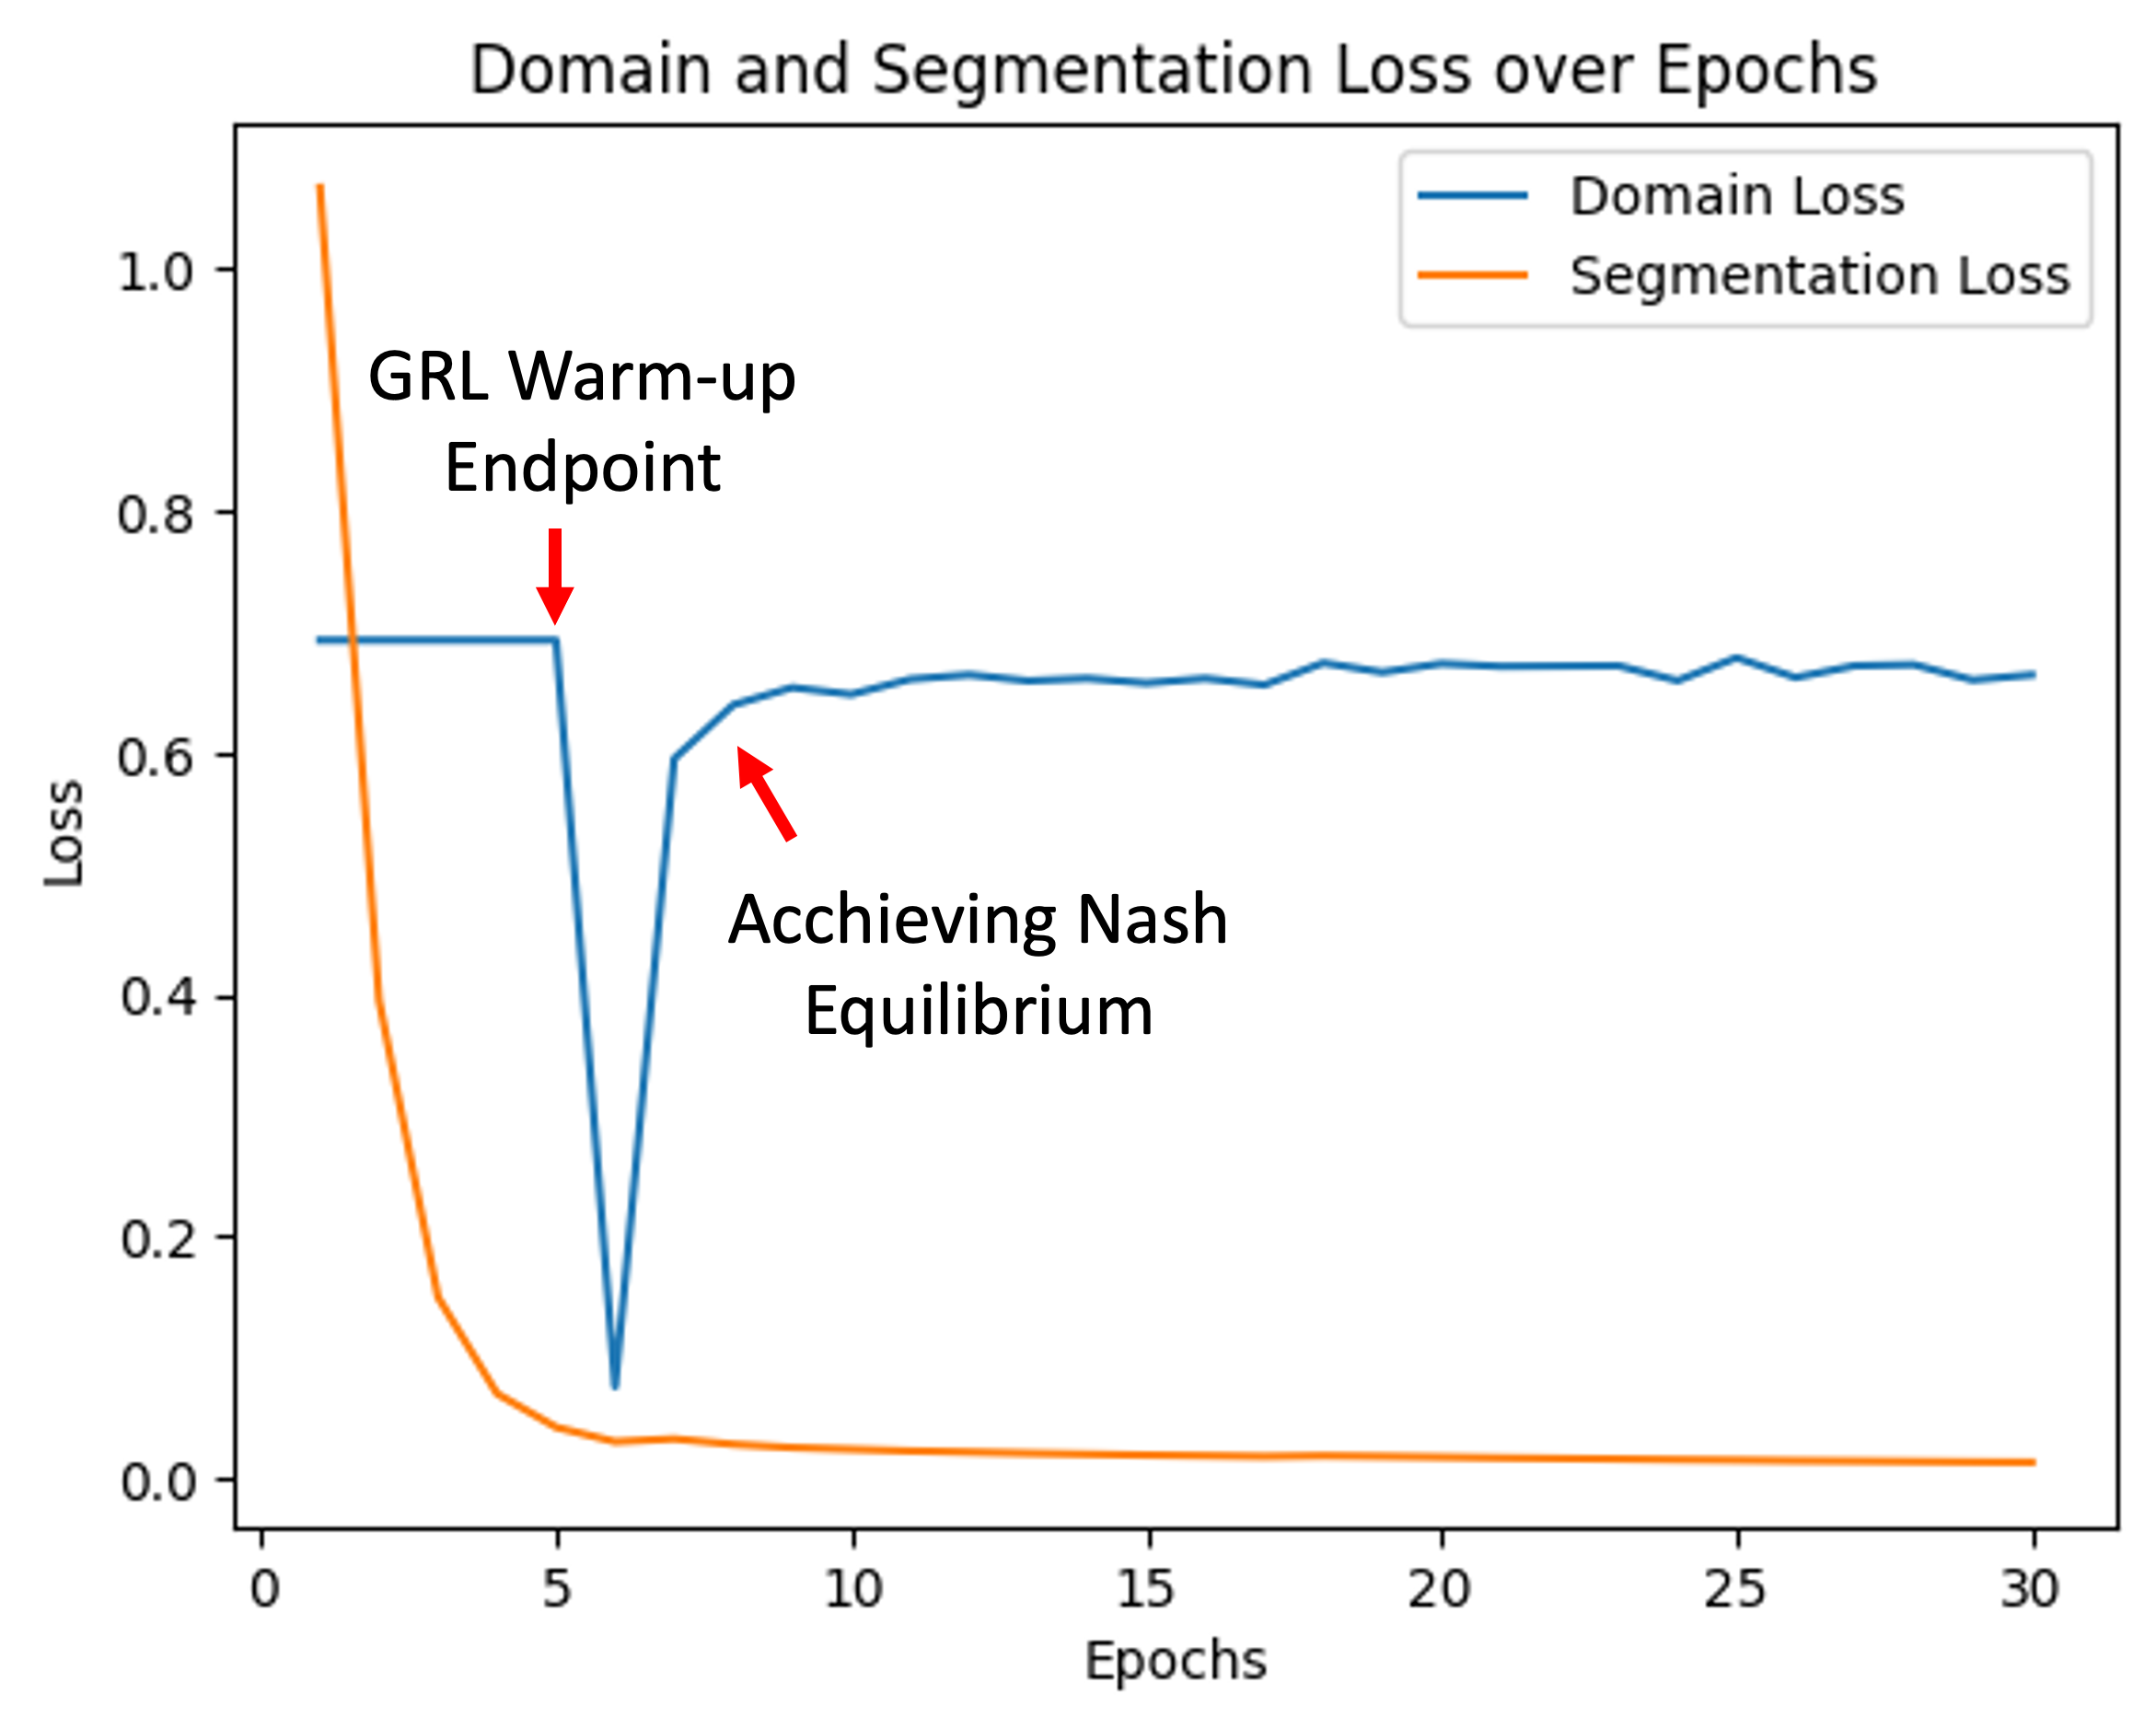
\includegraphics[width=0.8\linewidth]{figures/dann_loss.png}
        \caption{$L_{adv}$ 和 $L_{seg}$ 的动态变化曲线}
        \label{fig:dann_loss}
      \end{figure}
    \subsubsection{域判别损失的收敛状态分析}
      通过引入该动态冻结策略，本研究成功克服了常规 UDA 训练中常见的崩溃现象。
      在实际的训练监控中可以观察到，在二分类（源域 vs 目标域）的对抗博弈中，随着训练的深入，
      域判别损失（$L_{adv}$）不再持续趋近于 $0$，而是在 $0.693$（即 $-\ln(0.5)$）附近震荡。
      \par 对于二值交叉熵损失（Binary Cross-Entropy Loss），该数值对应域判别器难以稳定区分源域与目标域特征的状态。
      因此，这一现象说明动态冻结策略在训练过程中缓解了判别器过强带来的梯度失衡问题，并提示特征提取器在一定程度上削弱了 DESS 与 FSE 序列间的对比度差异。
      需要指出的是，域判别损失接近随机判别水平并不能单独证明特征完全域不变，其有效性仍需结合下游分割性能共同判断。
\section{本章实验与结果分析}
  为了验证上述改进型 DANN 网络架构及其动态对抗训练策略在临床无标注数据上的实际效能，
  本节在前期构建的人工标注测试集上进行了定量与定性分析，并对训练过程中的损失动力学进行了复盘。
  \subsection{UDA任务中判别器收敛过快导致生成器梯度消失}
    本章实验的基线模型（Baseline）设定为仅在源域（OAI-ZIB 的 DESS 序列）上进行全监督训练、而未施加任何域适应操作的标准 U-Net 模型。
    目标域的测试数据选取了人工精细标注的 150 张具有代表性的临床 FSE 序列切片。
    \par 在量化评估体系上，本研究主要采用以下两项空间重叠与距离度量指标：
    \begin{itemize}
      \item Dice 相似系数（Dice Similarity Coefficient, DSC）：用于衡量模型预测掩膜与人工 Ground Truth 在空间上的体积重叠率。其取值范围为 0 到 1。
      \item 平均表面距离（Average Surface Distance, ASD）：用于衡量模型预测掩膜与 Ground Truth 之间的平均边界距离，单位为毫米（mm）。ASD 越小表示分割边界越接近真实解剖结构。
      \item 根均方表面距离（Root Mean Square Surface Distance, RSD）：用于衡量模型预测掩膜与 Ground Truth 之间的边界距离的标准差，反映了分割边界的稳定性。
      \item 最大表面距离（Maximum Surface Distance, MSD）：用于衡量模型预测掩膜与 Ground Truth 之间的边界距离的最大值，反映了分割结果中最严重的错误。
    \end{itemize}
  \subsection{训练过程分析与域判别状态验证}
    动态冻结策略的训练曲线反映了域博弈的收敛轨迹。
    在训练的前 5 个 epoch 中，由于启动了 GRL 预热机制（$\lambda=0$），域判别器未接收对抗梯度，损失曲线保持相对平直，此时特征提取器迅速在源域数据上捕获了强语义特征。
    \par 在第 6 个 epoch 权重瞬间介入时，判别器立刻识别出了 DESS 与 FSE 序列间的巨大域差异，导致域损失发生陡降。
    然而，得益于本研究引入的动态损失比率监控机制（$\rho_t$），当判别器表现过强时，其参数更新被强制冻结。在随后的对抗训练中，生成器迅速追赶并拉近了两个域的分布。
    最终，域损失（Domain Loss）不再发散，而是在 $0.693$（即 $-\ln(0.5)$）附近震荡。
    这一现象表明域判别器难以持续稳定地区分源域和目标域特征，提示模型在一定程度上削弱了序列对比度风格差异；但该结论仍需结合目标域分割结果进行综合判断。
  \subsection{目标域分割结果的定量与定性分析}
    为了客观评估改进型 DANN 模型在跨域（从 OAI-ZIB 的 DESS 序列迁移至本地临床 FSE 序列）任务上的真实性能，本节在人工精细标注的独立目标域测试集上进行了严格的定量评价。
    评估指标选用了医学图像分割领域公认的 Dice 相似系数（DSC）以衡量体积重叠度，并结合平均表面距离（Average Surface Distance, ASD）、根均方表面距离（Root Mean Square Surface Distance, RSD）以及最大表面距离（Maximum Surface Distance, MSD）来全面衡量边界的几何预测偏差。
    \subsubsection{定量评估结果}
      模型在目标域验证集上的各项定量指标统计如下表所示：
      \begin{table}[!hpt]
        \caption{基于改进型 DANN 的无监督域适应分割结果（平均值 ± 标准差）}
        \label{tab:dann_results}
        \centering
        \begin{tabular}{ccccc}
          \toprule
            标签 & DSC & ASD(mm) & RSD(mm) & MSD(mm) \\
          \midrule
            FB（股骨） & $0.9557 \pm 0.0243$ & $1.039 \pm 0.560$ & $1.697 \pm 0.947$ & $5.708 \pm 2.749$ \\
            FC（股骨软骨） & $0.7748 \pm 0.0633$ & $0.961 \pm 0.477$ & $2.161 \pm 1.237$ & $10.496 \pm 5.321$ \\
            TB（胫骨） & $0.9678 \pm 0.0231$ & $0.547 \pm 0.340$ & $0.873 \pm 0.611$ & $3.236 \pm 2.521$ \\
            TC（胫骨软骨） & $0.7530 \pm 0.1505$ & $0.678 \pm 0.553$ & $1.268 \pm 0.937$ & $5.801 \pm 3.184$ \\
          \bottomrule
        \end{tabular}
      \end{table}
    \subsubsection{骨骼分割性能分析（FB与TB）}
      由表可知，模型在大型骨性结构（股骨 FB 与胫骨 TB）的分割上展现出了较好的跨域泛化能力。
      胫骨和股骨的平均 Dice 系数分别达到了 \num{0.9678} 和 \num{0.9557}，且平均表面距离（ASD）均控制在 \qty{1}{\milli\metre} 左右（胫骨更是低至 \qty{0.547}{\milli\metre}）。
      这表明，尽管源域 DESS 序列与目标域 Fat-suppressed FSE 序列在骨髓信号上存在巨大的“风格”差异，但改进型 DANN 网络凭借实例归一化（IN）机制和动态对抗博弈，
      成功滤除了底层灰度分布差异与骨髓水肿的信号干扰，精准抓取了刚性骨骼的解剖学拓扑边界。
    \subsubsection{软骨分割性能分析（FC与TC）}
      关节软骨由于其极薄的曲面物理特性、在全图中极小的体素占比，且在不同 MRI 序列间的组织对比度变化剧烈，一直是无监督域适应（UDA）任务中的核心难点。
      在完全没有目标域软骨标签参与网络训练的苛刻条件下，本模型对股骨软骨（FC）和胫骨软骨（TC）的 Dice 系数分别达到了 \num{0.7748} 和 \num{0.7530}。
      \par 更具临床价值的是，软骨的平均表面距离（ASD）分别被严格限制在 \qty{0.961}{\milli\metre} 和 \qty{0.678}{\milli\metre}。
      考虑到临床常规 FSE 序列本身存在的部分容积效应，能够在未经本地数据监督的情况下达到亚毫米级的平均边界误差，
      说明 ASPP 模块可能有助于扩大感受野并保留局部边缘特征。
      这为后续章节基于掩膜提取软骨三维厚度与计算关节接触面积提供了可用的几何基础。
    \subsubsection{局部边界偏差与极端误差分析}
      值得注意的是，虽然整体的体积重叠率（DSC）与平均边界表现（ASD）优异，但最大表面距离（MSD）指标揭示了模型在局部极端解剖场景下的局限性。
      例如，股骨软骨（FC）的 MSD 达到了 \qty{10.496}{\milli\metre} $\pm$ \qty{5.321}{\milli\metre}，标准差相对较大。
      由于 MSD 测量的是预测边界与真实边界之间的最大单点距离，它对孤立的离群点（Outliers）极其敏感。
      \par 这种局部预测偏移通常发生在以下复杂场景中：
      \begin{itemize}
        \item 视野边缘与部分容积效应：在股骨髁的内外侧极边缘，或切片首尾处，软骨极度变薄，且受 Z 轴分辨率限制变得模糊，导致网络偶发性地产生孤立的假阳性像素斑块。
        \item 高能创伤与病理特征的干扰：本数据集中的孤立性 ACL 撕裂患者常伴有剧烈的局灶性骨挫伤（BML）以及高信号的关节腔积液。当积液与软骨表面紧密贴合时，缺乏组织对比度梯度，导致 DANN 在该局部区域未能精确对齐域不变特征，从而产生了少量的边界外溢。
      \end{itemize}
      \par 综合上述多维量化指标，本章所提出的改进型 DANN 架构在目标域 FSE 数据上获得了较好的骨骼与软骨分割表现。
      但由于二维单平面分析的固有缺陷，局部仍存在一定的最大表面距离（MSD）极值，这提示后续仍有必要引入三维空间融合（如第五章所述的 DIP 高分辨率重建）来增强三维解剖连续性约束。







